\documentclass{beamer}
\usepackage{TDH-macros}
\usepackage{graphicx}

\newcommand{\neff}{\text{popsize}}
\newcommand{\aij}{\alpha_{ij}(t)}
\newcommand{\aijs}{\alpha_{ij}^*(t)}
\newcommand{\wij}[1]{w_{ij}^{\text{#1}}}


\AtBeginSection[]
{
  \begin{frame}<beamer>
    \frametitle{Outline}
    \tableofcontents[currentsection]
  \end{frame}
}

\AtBeginSubsection[]
{
  \begin{frame}<beamer>
    \frametitle{Outline}
    \tableofcontents[currentsection,currentsubsection]
  \end{frame}
}

\begin{document}

\title{Simulation and modeling of genomic signatures of selection in
  order to identify functional genes in domestic animals} \author{Toby
  Dylan Hocking} \date{17 June 2009} \institute{INRA Jouy-en-Josas,
  G\'en\'etique Animale et Biologie Int\'egrative}

\frame{\titlepage}

\newcommand{\framet}[2]{\frame{
\begin{itemize}
\frametitle{#1}{#2}
\end{itemize}
}}

\newcommand{\picframe}[1]{
  \frame[plain]{
    \includegraphics[width=\textwidth]{#1}
  }
}

\section{Education, work experience, qualifications, and interests}

\framet{Education and internships 2002-2006}{
\item Bachelor of Arts, University of California, Berkeley, May 2006
\begin{itemize}
  \item Major in Molecular and Cell Biology, emphasis Genetics and Development
  \item Major in Statistics, with honors thesis for research with
    Dr. Terry Speed on chromosomal copy number analysis on Single
    Nucleotide Polymorphism (SNP) microarray data
\end{itemize}
\item Research internships
\begin{itemize}
\item Expression microarray analysis, Lawrence Berkeley National
  Laboratory (LBNL), with Dr. Saira Mian, 2003-2004
\item Human tissue culture and molecular biology, LBNL, with Dr. Chris
  Patil, 2004
\item Fungal genetics, Genencor International, with Dr. Huaming Wang, 2005
\end{itemize}
}

\framet{Work experience 2006-2008}{
\item Research assistant at Sangamo BioSciences, with Dr. Jeff Miller
\begin{itemize}
\item Biochemistry experiments to determine DNA-binding sequnces of zinc finger proteins
\item Doyon Y, McCammon JM, Miller JC, Faraji F, Ngo C, Katibah GE,
  Amora R, \textbf{Hocking TD}, Zhang L, Rebar EJ, Gregory PD, Urnov
  FD, Amacher SL. Heritable targeted gene disruption in zebrafish
  using designed zinc-finger nucleases, \emph{Nature Biotechnology}
  26, 702-708 (2008).
\item Designed linker sequences for chimeric nucleases and tested their specificity and activity using a yeast reporter system
\item Implemented an interactive database/webserver for statistical
  analysis and visualization (open sourced a plotting framework)
\end{itemize}
}

\framet{Skills, current work 2008-2009}{
\item Language skills: English (mother tongue) and French (spoken since 2007, living in Paris since August 2008)
\item Programming skills: C, Perl, Python, R, SAS, HTML, SQL, PHP, CSS, \LaTeX, Subversion
\item Master 2 Statistics at University of Pierre and Marie
  Curie, Paris 6, director Paul Deheuvels
\item Currently doing a research internship with Drs. Mathieu Gautier,
  Jean-Louis Foulley, and Gilles Celeux at INRA/INRIA
}

\section{Genomic differentiation and selection of domestic animals}

\framet{Need to identify functional genes motivates study of domestic animals}{
\item The Bovine Genome Sequencing and Analysis Consortium, Christine
  G. Elsik, Ross L. Tellam, Kim C. Worley, et al. The Genome Sequence
  of Taurine Cattle: A Window to Ruminant Biology and Evolution,
  \emph{Science}, 2009 Apr 24; 324:522-528.
\item Domestic animals (not just cows) have been subjected to
  domestication and natural selection for thousands of years.
\item Selection of favorable phenotypes: resistance to disease, milk
  production, meat production, etc.
\item How can we characterize the genomic regions and genes that
  correspond to this selection?
\item Example: climate change may introduce an African disease to
  Europe, we would like to identify which genes in African cattle are
  responsible for resistance.
}

\framet{Toward a signature of selection}{
\item We can inexpensively genotype a cow at 60,000 SNPs using
  microarrays, and compare these genotypes between modern domestic
  populations.
\item The question: can we derive a statistic -- a ``signature of
  selection'' -- that indicates a genomic region has been under
  selection?
}

\picframe{evolution}

\framet{Models of evolution and genetic differentiation}{
\item 4 evolutive forces: drift, selection, migration, and mutation.
\item Several types of selection:
\item Positive selection acts to favor homozygotes, thus increasing
  the allele frequency.
\item Balancing selection favors heterozygotes, thus tending to
  maintain several favorable alleles, evolving allele frequencies
  towards 1/2.
\item The ``signature of selection'' will enable identification of loci
  under selection and estimation of the strength of selection.
}

\framet{Bayesian statistical models of evolution}{
\item Hierarchical Bayesian models offer a robust framework for
  studying genetics.
\item Models can be fit using Markov Chain Monte Carlo (MCMC)
  techniques.
\item Some current models work well but only consider drift (Nicholson
  \etal\ 2002).
\item Examine which loci do not fit, to infer which loci are not
  consistent with the pure-drift model.
\item Some other models attempt to estimate selection coefficients
  (Beaumont and Balding 2004).
\item With more complex genetic models of evolution (selection,
  migration), our statistical models become less tractable.
\item In very complex genetic models (Kimura equations) it is
  impossible to write the likelihood.
\item But we can still simulate the data, so potentially can use
  Approximate Bayesian Computation (ABC).  }

\framet{Conclusion: steps toward a signature of selection}{
\item Introduce parameters for selection into a hierarchical Bayesian
  model.
\item Design a per-locus ``signature of selection'' for behavior
  different than a neutral allele.
\item Most current models assume independence of loci, which is false.
\item Use Approximate Bayesian Computation (ABC) to estimate selection
  parameters when it is impossible to write the likelihood.
\item Model the ascertainment bias inherent in microarray design.
}


\framet{Merci pour votre attention}{
  \item Questions?
}

\framet{}{\item Supplementary slides follow}

\framet{Why Bayesian models?}{
\item Structured way to model different sources of variation
\item Posterior distributions (and credible interval) for parameters, rather than point
estimates
\item Hierarchical structure for shrinkage of parameters towards zero (= sparsity assumption)
\item Can be computationally efficient through empirical Bayesian approach
\item Incorporate biological information into priors
\item Avoid overfitting that occurs with ML methods 
}

\framet{A simple selection simulator, based on Beaumont, Balding (2004)}{
\item Simulate the evolution using known evolution parameters, fit the
  model, then look for signatures of selection in the alleles we know
  were under selection.
\item Single ancestral population.
\item Several subpopulations:
  \begin{itemize}
  \item Initially with the same allele frequency but evolving
    independently.
  \item Each has a different background color (blue, red, neutral).
  \end{itemize}
\item Several independent loci:
  \begin{itemize}
  \item Two alleles (red, blue) to mimic the SNP data.
  \item Each has a different selection coefficient $s\in \RR^+$, but
    normally in reality $s<1$.
  \item Each has a different selection type (neutral, positive, or balancing).
  \end{itemize}
\item Evolution by drift and selection over several generations.
 }

\framet{Evolution equations}{
\item locus $i$, population $j$, time $t$
\item blue allele frequency $\alpha_{ij}(t)$
\item genetic drift $\aijs = \operatorname{rbinom}(\neff,\alpha_{ij}(t-1))/\neff$
\item relative fitness of genotypes 
$$
\begin{array}{cccll}
\wij{BB} & \wij{BR} & \wij{RR} & i & j\\
\hline
1 & 1+s_i/2 & 1+s_i & \text{positive}& \text{red}\\
1+s_i & 1+s_i/2 & 1 & \text{positive}& \text{blue}\\
1 & 1+s_i & 1 & \text{balancing}& \\
1 & 1 & 1 & \text{neutral}& 
\end{array}
$$
\item allele frequency updated for selection based on Hardy-Weinberg equilibrium:
$$\aij = \frac{
\wij{BB}\aijs^2 + \wij{BR}\aijs[1-\aijs]/2 }{
\wij{BB}\aijs^2 + \wij{BR}\aijs[1-\aijs] + \wij{RR}[1-\aijs]^2
   }$$
}

\framet{The hierarchical bayesian Nicholson model}{
\item number of alleles $x_{ij}\sim \Bin(\neff,\alpha_{ij})$
\item subpopulation allele frequency $\alpha_{ij}\sim N(\pi_i, c_j \pi_i(1-\pi_i))$
\item ancestral allele frequency prior $\pi_i\sim \beta(a,a)$
\item \textbf{population differentiation prior $c_j\sim U[0,1]$}
\item Monte Carlo Markov Chain sampling: 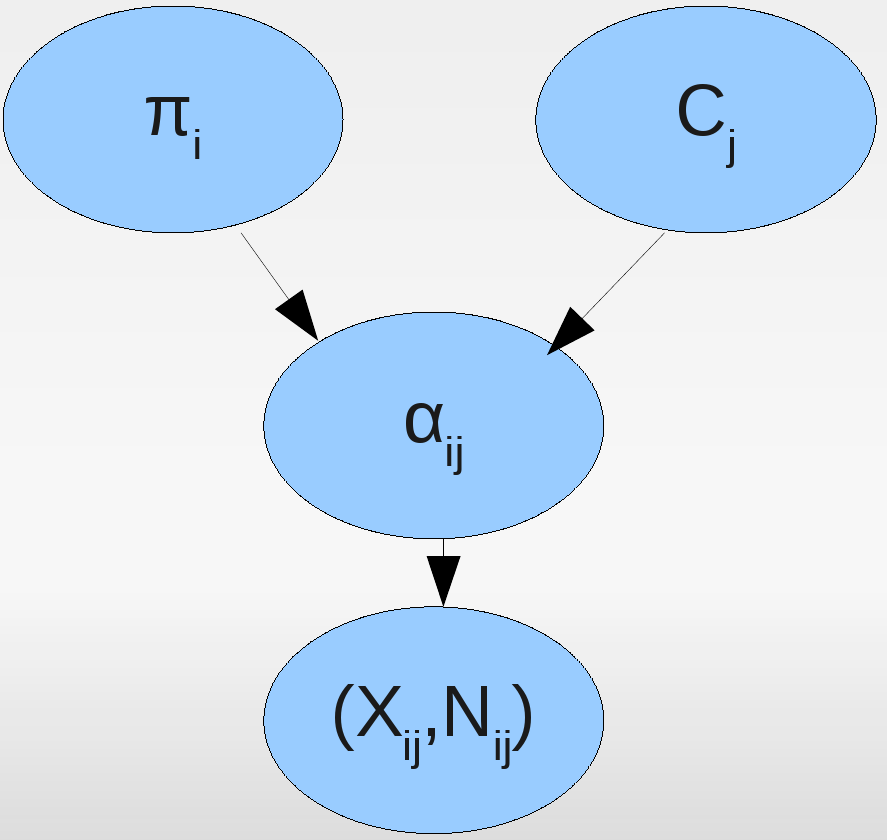
\includegraphics[width=0.2\textwidth]{nicholson-model}
\begin{enumerate}
\item $\alpha^t = P(\alpha|c^{t-1},\pi^{t-1},x)$
\item $\pi^t = P(\pi|c^{t-1},\alpha^t,a)$
\item $c^t = P(c|\pi^t,\alpha^t)$
\end{enumerate}
\item Implemented using a Gibbs sampler in a FORTRAN program.
}

\picframe{abc}



\end{document}